\documentclass[UTF8]{article}

\usepackage{ctex}
\usepackage{amsmath}
\usepackage{amssymb}
\usepackage{amsthm}
\providecommand{\abs}[1]{\lvert#1\rvert}
\providecommand{\norm}[1]{\lVert#1\rVert}

\newtheorem{thm}{Theorem}
\newtheorem{lemma}[thm]{Lemma}
\newtheorem{fact}[thm]{Fact}
\newtheorem{cor}[thm]{Corollary}
\newtheorem{eg}{Example}
\newtheorem{ex}{Exercise}
\newtheorem{defi}{Definition}
\newtheorem{hw}{Problem}
\newenvironment{sol}

  {\par\vspace{3mm}\noindent{\it Solution}.}


\usepackage{algorithm,algorithmic,bm,color}
\floatstyle{plain}
\newfloat{myalgo}{tbhp}{mya}
\newenvironment{Algorithm}[2][tbh]
{\begin{myalgo}[#1]\centering\begin{minipage}{#2}\begin{algorithm}[H]}%
{\end{algorithm}\end{minipage}\end{myalgo}}

% Use the postscript times font!
\usepackage{times}
\usepackage{soul}
\usepackage{url}
\usepackage[hidelinks]{hyperref}
\usepackage[utf8]{inputenc}
\usepackage[small]{caption}
\usepackage{graphicx}
\usepackage{amsmath}
\usepackage{booktabs}
\usepackage{algorithm}
\usepackage{algorithmic}\usepackage{amsfonts}
\urlstyle{same}

\makeatletter

\makeatother

\setlength{\parindent}{0pt}

%\setlength{\parskip}{2ex}

\newenvironment{proofof}[1]{\bigskip\noindent{\itshape #1. }}{\hfill$\Box$\medskip}
\usepackage{enumerate,fullpage,proof}



% the following package is optional:

%\usepackage{latexsym} 

\usepackage{amsfonts}
\usepackage{subfigure}
\usepackage{booktabs}
\usepackage{stfloats}
\usepackage{amssymb}
\DeclareMathOperator{\diag}{diag}
\DeclareMathOperator{\mst}{s.t.}
\DeclareMathOperator{\var}{Var}
\DeclareMathOperator{\cov}{Cov}
\renewcommand{\algorithmicrequire}{\textbf{Input:}}
\renewcommand{\algorithmicensure}{\textbf{Output:}}


\newcommand{\argmin}{\arg\!\min}
\newcommand{\argmax}{\arg\!\max}
\newcommand{\Amat}{{\boldsymbol A}}
\newcommand{\Bmat}{{\boldsymbol B}}
\newcommand{\Cmat}{{\boldsymbol C}}
\newcommand{\Dmat}{{\boldsymbol D}}
\newcommand{\Emat}[0]{{{\boldsymbol E}}}
\newcommand{\Fmat}[0]{{{\boldsymbol F}}}
\newcommand{\Gmat}[0]{{{\boldsymbol G}}}
\newcommand{\Hmat}[0]{{{\boldsymbol H}}}
\newcommand{\Imat}{{\boldsymbol I}}
\newcommand{\Jmat}[0]{{{\boldsymbol J}}}
\newcommand{\Kmat}[0]{{{\boldsymbol K}}}
\newcommand{\Lmat}[0]{{{\boldsymbol L}}}
\newcommand{\Mmat}[0]{{{\boldsymbol M}}}
\newcommand{\Nmat}[0]{{{\boldsymbol N}}}
\newcommand{\Omat}[0]{{{\boldsymbol O}}}
\newcommand{\Pmat}[0]{{{\boldsymbol P}}}
\newcommand{\Qmat}[0]{{{\boldsymbol Q}}}
\newcommand{\Rmat}[0]{{{\boldsymbol R}}}
\newcommand{\Smat}[0]{{{\boldsymbol S}}}
\newcommand{\Tmat}[0]{{{\boldsymbol T}}}
\newcommand{\Umat}{{{\boldsymbol U}}}
\newcommand{\Vmat}[0]{{{\boldsymbol V}}}
\newcommand{\Wmat}[0]{{{\boldsymbol W}}}
\newcommand{\Xmat}{{\boldsymbol X}}
\newcommand{\Ymat}[0]{{{\boldsymbol Y}}}
\newcommand{\Zmat}{{\boldsymbol Z}}

\newcommand{\av}{\boldsymbol{a}}
\newcommand{\Av}{\boldsymbol{A}}
\newcommand{\Cv}{\boldsymbol{C}}
\newcommand{\bv}{\boldsymbol{b}}
\newcommand{\cv}{{\boldsymbol{c}}}
\newcommand{\dv}{\boldsymbol{d}}
\newcommand{\ev}[0]{{\boldsymbol{e}}}
\newcommand{\fv}{\boldsymbol{f}}
\newcommand{\Fv}[0]{{\boldsymbol{F}}}
\newcommand{\gv}[0]{{\boldsymbol{g}}}
\newcommand{\hv}[0]{{\boldsymbol{h}}}
\newcommand{\iv}[0]{{\boldsymbol{i}}}
\newcommand{\jv}[0]{{\boldsymbol{j}}}
\newcommand{\kv}[0]{{\boldsymbol{k}}}
\newcommand{\lv}[0]{{\boldsymbol{l}}}
\newcommand{\mv}[0]{{\boldsymbol{m}}}
\newcommand{\nv}{\boldsymbol{n}}
\newcommand{\ov}[0]{{\boldsymbol{o}}}
\newcommand{\pv}[0]{{\boldsymbol{p}}}
\newcommand{\qv}[0]{{\boldsymbol{q}}}
\newcommand{\rv}[0]{{\boldsymbol{r}}}
\newcommand{\sv}[0]{{\boldsymbol{s}}}
\newcommand{\tv}[0]{{\boldsymbol{t}}}
\newcommand{\uv}[0]{{\boldsymbol{u}}}
\newcommand{\vv}{\boldsymbol{v}}
\newcommand{\wv}{\boldsymbol{w}}
\newcommand{\Wv}{\boldsymbol{W}}
\newcommand{\xv}{\boldsymbol{x}}
\newcommand{\yv}{\boldsymbol{y}}
\newcommand{\Xv}{\boldsymbol{X}}
\newcommand{\Yv}{\boldsymbol{Y}}
\newcommand{\zv}{\boldsymbol{z}}
\newcommand{\xvf}{\widetilde{\xv}}
\newcommand{\Fmb}{\boldsymbol{\mathcal{F}}}
\newcommand{\Gammamat}[0]{{\boldsymbol{\Gamma}}}
\newcommand{\Deltamat}[0]{{\boldsymbol{\Delta}}}
\newcommand{\Thetamat}{\boldsymbol{\Theta}}
\newcommand{\Lambdamat}{{\boldsymbol{\Lambda}}}
\newcommand{\Ximat}[0]{{\boldsymbol{\Xi}}}
\newcommand{\Pimat}[0]{{\boldsymbol{\Pi}} }
\newcommand{\Sigmamat}{\boldsymbol{\Sigma}}
\newcommand{\Upsilonmat}[0]{{\boldsymbol{\Upsilon}} }
\newcommand{\Phimat}{\boldsymbol{\Phi}}
\newcommand{\Psimat}{\boldsymbol{\Psi}}
\newcommand{\Omegamat}{{\boldsymbol{\Omega}}}
\newcommand{\Lambdav}{\bm{\Lambda}}
\newcommand{\alphav}{\boldsymbol{\alpha}}
\newcommand{\betav}[0]{{\boldsymbol{\beta}} }
\newcommand{\gammav}{{\boldsymbol{\gamma}}}
\newcommand{\deltav}[0]{{\boldsymbol{\delta}} }
\newcommand{\epsilonv}{\boldsymbol{\epsilon}}
\newcommand{\zetav}[0]{{\boldsymbol{\zeta}} }
\newcommand{\etav}[0]{{\boldsymbol{\eta}} }
\newcommand{\thetav}{\boldsymbol{\theta}}
\newcommand{\iotav}[0]{{\boldsymbol{\iota}} }
\newcommand{\kappav}{{\boldsymbol{\kappa}}}
\newcommand{\lambdav}[0]{{\boldsymbol{\lambda}} }
\newcommand{\muv}{\boldsymbol{\mu}}
\newcommand{\nuv}{{\boldsymbol{\nu}}}
\newcommand{\xiv}{{\boldsymbol{\xi}}}
\newcommand{\omicronv}[0]{{\boldsymbol{\omicron}} }
\newcommand{\piv}{\boldsymbol{\pi}}
\newcommand{\rhov}[0]{{\boldsymbol{\rho}} }
\newcommand{\sigmav}[0]{{\boldsymbol{\sigma}} }
\newcommand{\tauv}[0]{{\boldsymbol{\tau}} }
\newcommand{\upsilonv}[0]{{\boldsymbol{\upsilon}} }
\newcommand{\phiv}{\boldsymbol{\phi}}
\newcommand{\chiv}[0]{{\boldsymbol{\chi}} }
\newcommand{\psiv}{\boldsymbol{\psi}}
\newcommand{\omegav}[0]{{\boldsymbol{\omega}} }
\newcommand{\tsp}{^{\mathsf{T}}}
\newcommand{\inv}{^{-1}}
\newcommand{\ie}{{\em i.e.}}
\newcommand{\wrt}{{\em w.r.t.\,}}
\begin{document}

\begin{center}
{\LARGE\bf 第三次作业}
\end{center}

\begin{hw}
SVM vs Neural Network
\begin{sol}
	比较SVM和Neural Network在不同数据集上的判别能力。按照要求从两个网站选定了三个数据集:iris,colon-cancer和mnist\cite{dataset,dpdataset}。
	\begin{enumerate}
		\item[(1)]{
			首先是iris数据集,该数据集提供了鸢尾花的多个特征,并根据他们对鸢尾花进行分类。表\ref{tab:iris}中展示的是一个两个隐藏层的使用relu激活的多层感知机和核函数为多项式,C为0.01的SVM,他们在测试集上的准确率均为100\%。在这样一个特征维度并不高的数据集上,训练集充分,两种模型均可以学到极好的分类能力。图\ref{fig:a1svm}和图\ref{fig:a1nn}展示了各个参数下的SVM和MLP的测试结果。
			
	
			\begin{figure}[htbp]
				\centering
				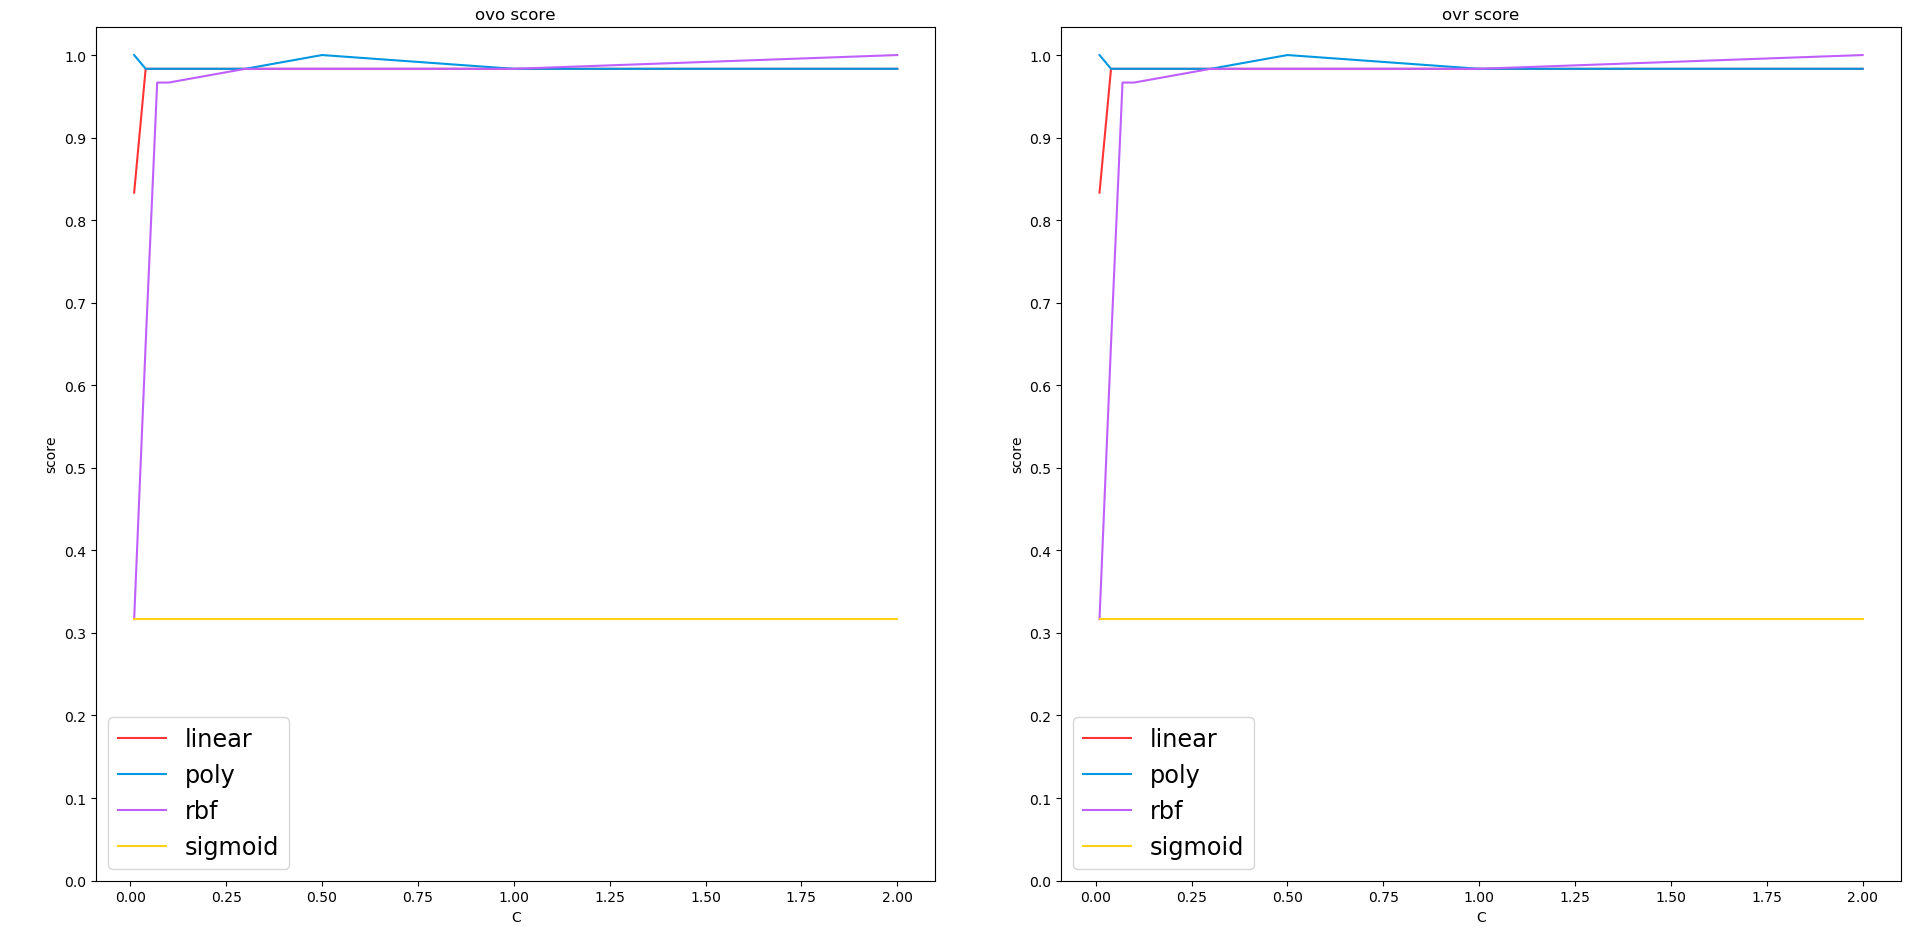
\includegraphics[width=0.5\linewidth]{figure/a1_svm}
				\caption{Iris数据集上的SVM表现。}
				\label{fig:a1svm}
			\end{figure}		
			\begin{figure}[htbp]
				\centering
				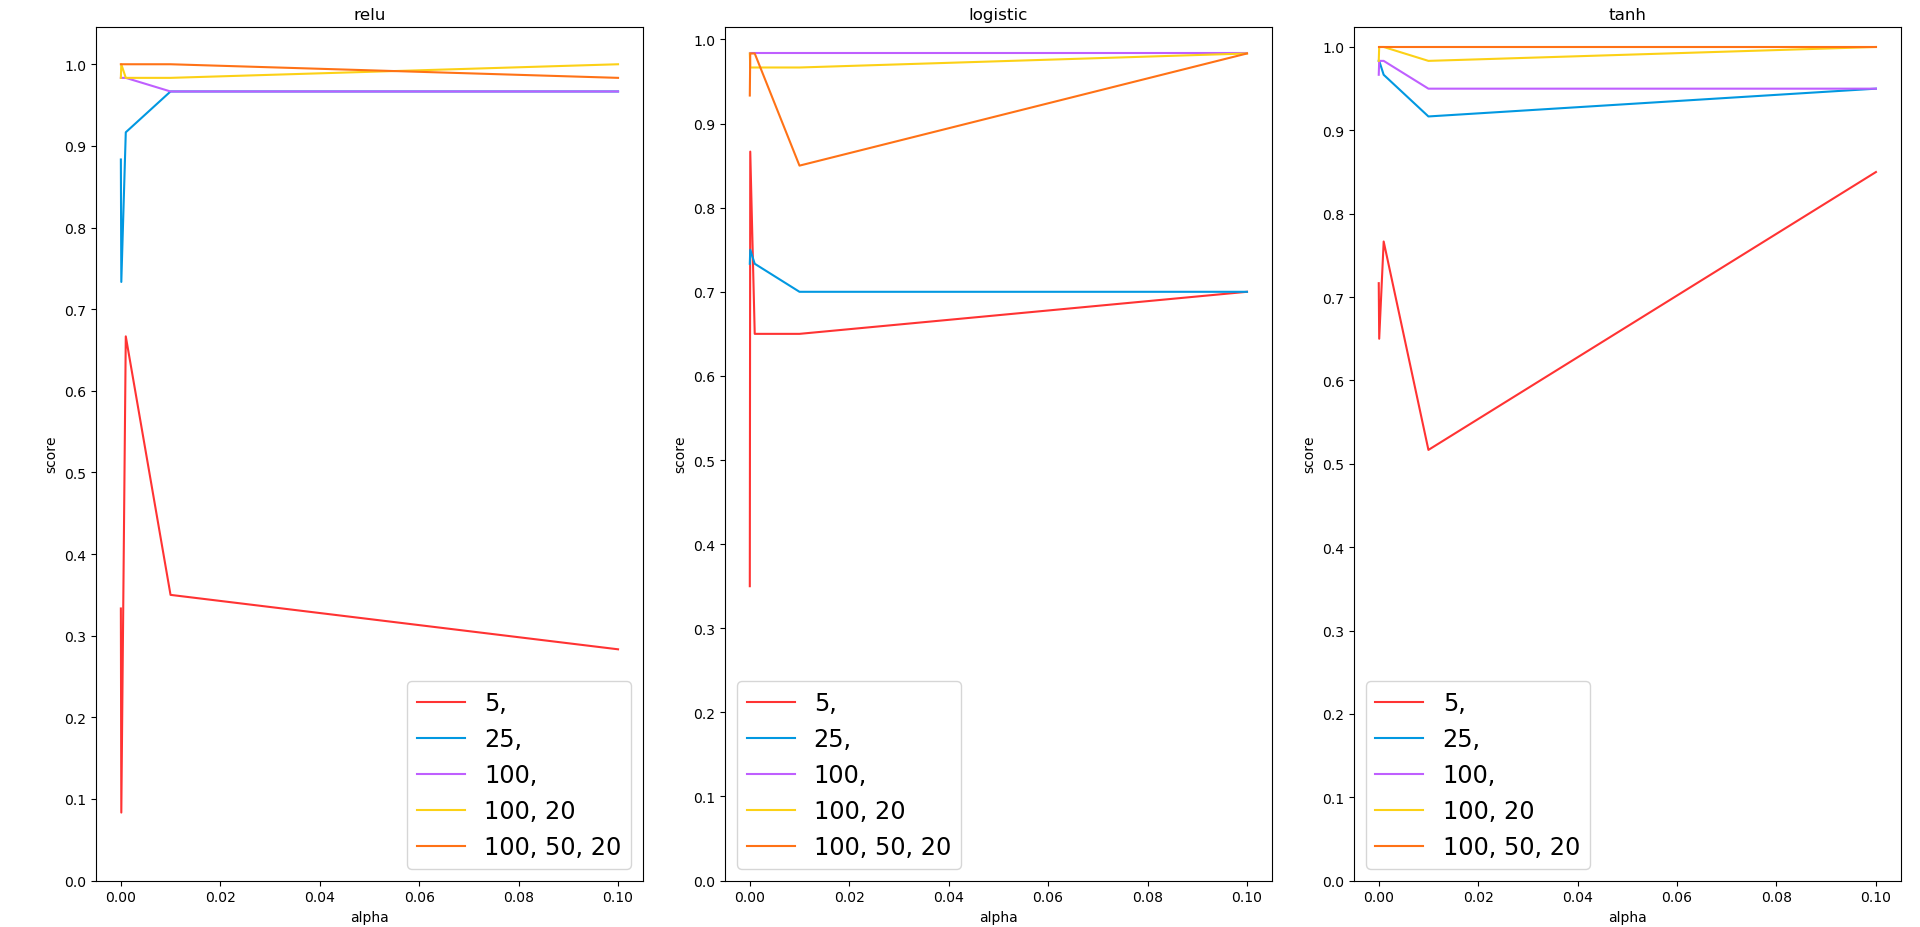
\includegraphics[width=0.5\linewidth]{figure/a1_nn}
				\caption{Iris数据集上的MLP表现。}
				\label{fig:a1nn}
			\end{figure}
			
			\begin{table}[htbp]
				\centering
				\small
				\caption{Iris上的准确率比较。}
				\label{tab:iris}
				\begin{tabular}{lr}
					\toprule
					方法 & 准确率       \\ \midrule
					MLP(relu,0.001,100$\times$20)  & 99.77\%  \\ %\midrule
					SVM(polynomial kernel with C=0.01) 	  & 100\%  \\
					\bottomrule
				\end{tabular}
				\vspace{-5mm}
			\end{table}	
		}
	
		\item[(2)]{
			Colon cancer数据集提供了结肠癌患者和普通患者的数据,希望二分类问题,即患者是否患有结肠癌症。表\ref{tab:colon}中核函数为sigmoid函数,C为2时,准确率可以达到84\%;而多层感知机,由于该数据集上训练集数量较小,由于我们设置的维度较大,都未能收敛,仅有10\%的准确度,成了反向的分类器。图\ref{fig:a2svm}和图\ref{fig:a2nn}展示了各个参数下的SVM和MLP的测试结果。
			
			\begin{figure}[htbp]
				\centering
				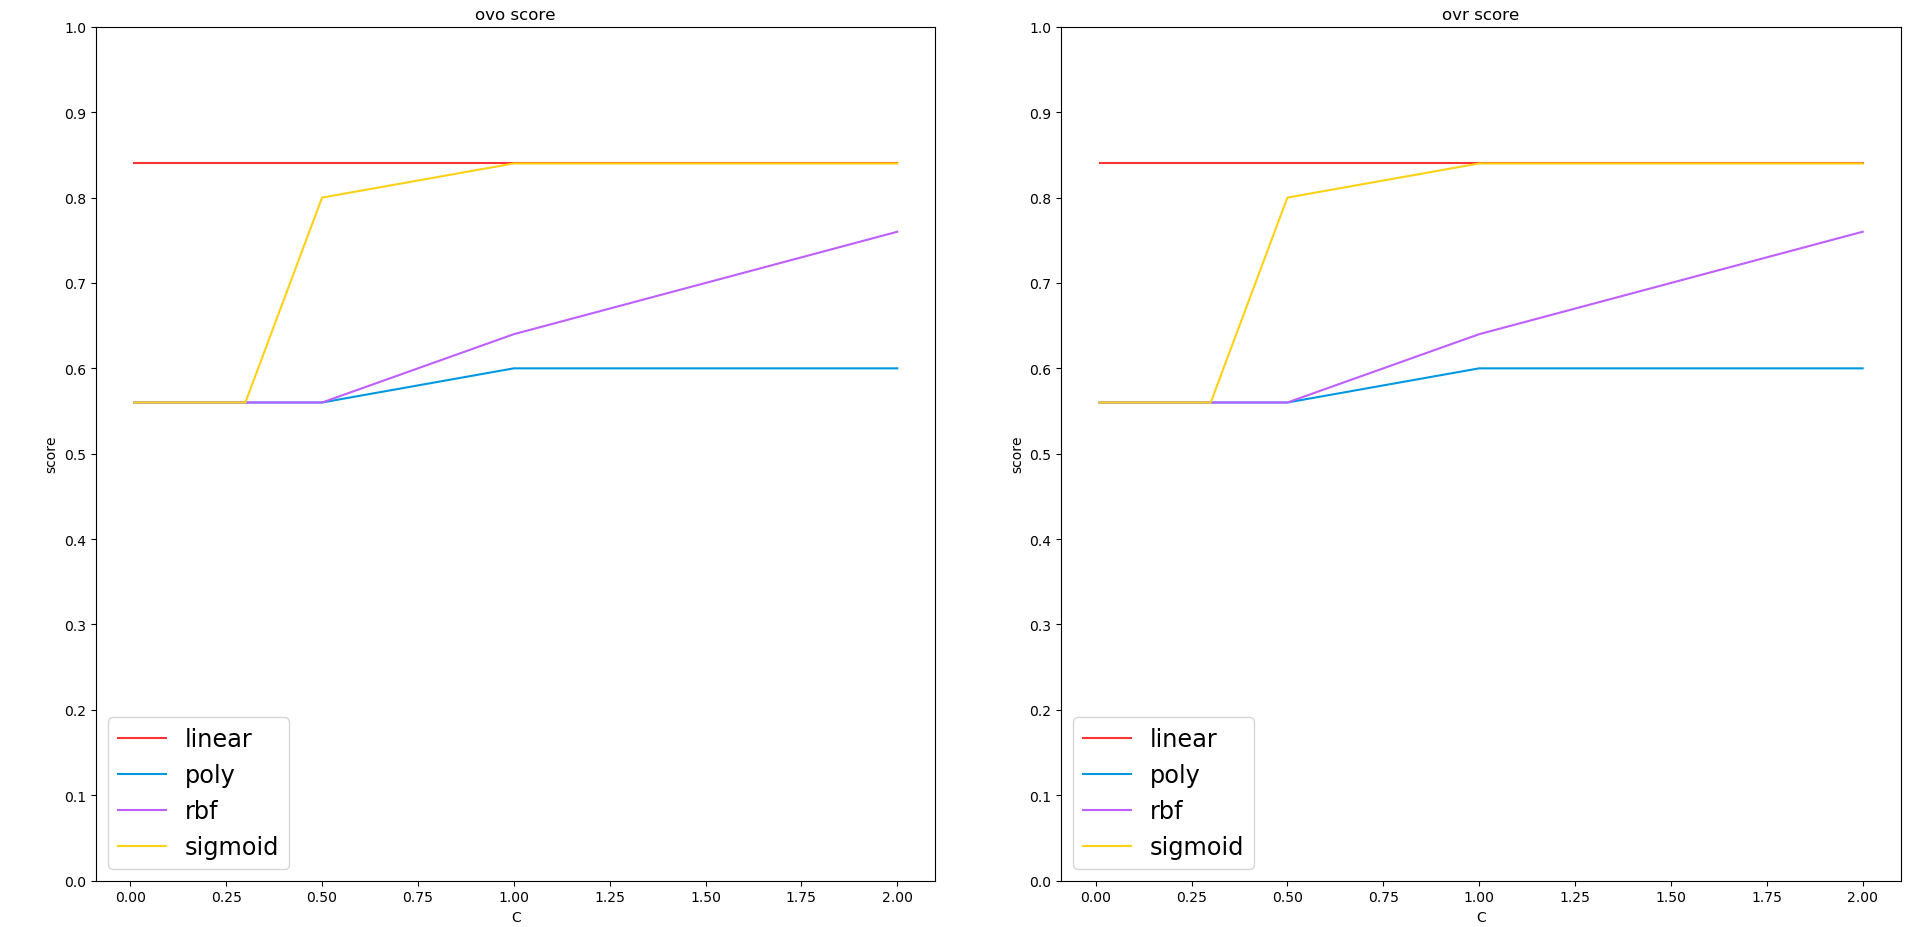
\includegraphics[width=0.5\linewidth]{figure/a2_svm}
				\caption{Colon Cancer数据集上的SVM表现。}
				\label{fig:a2svm}
			\end{figure}
			
			\begin{figure}[htbp]
				\centering
				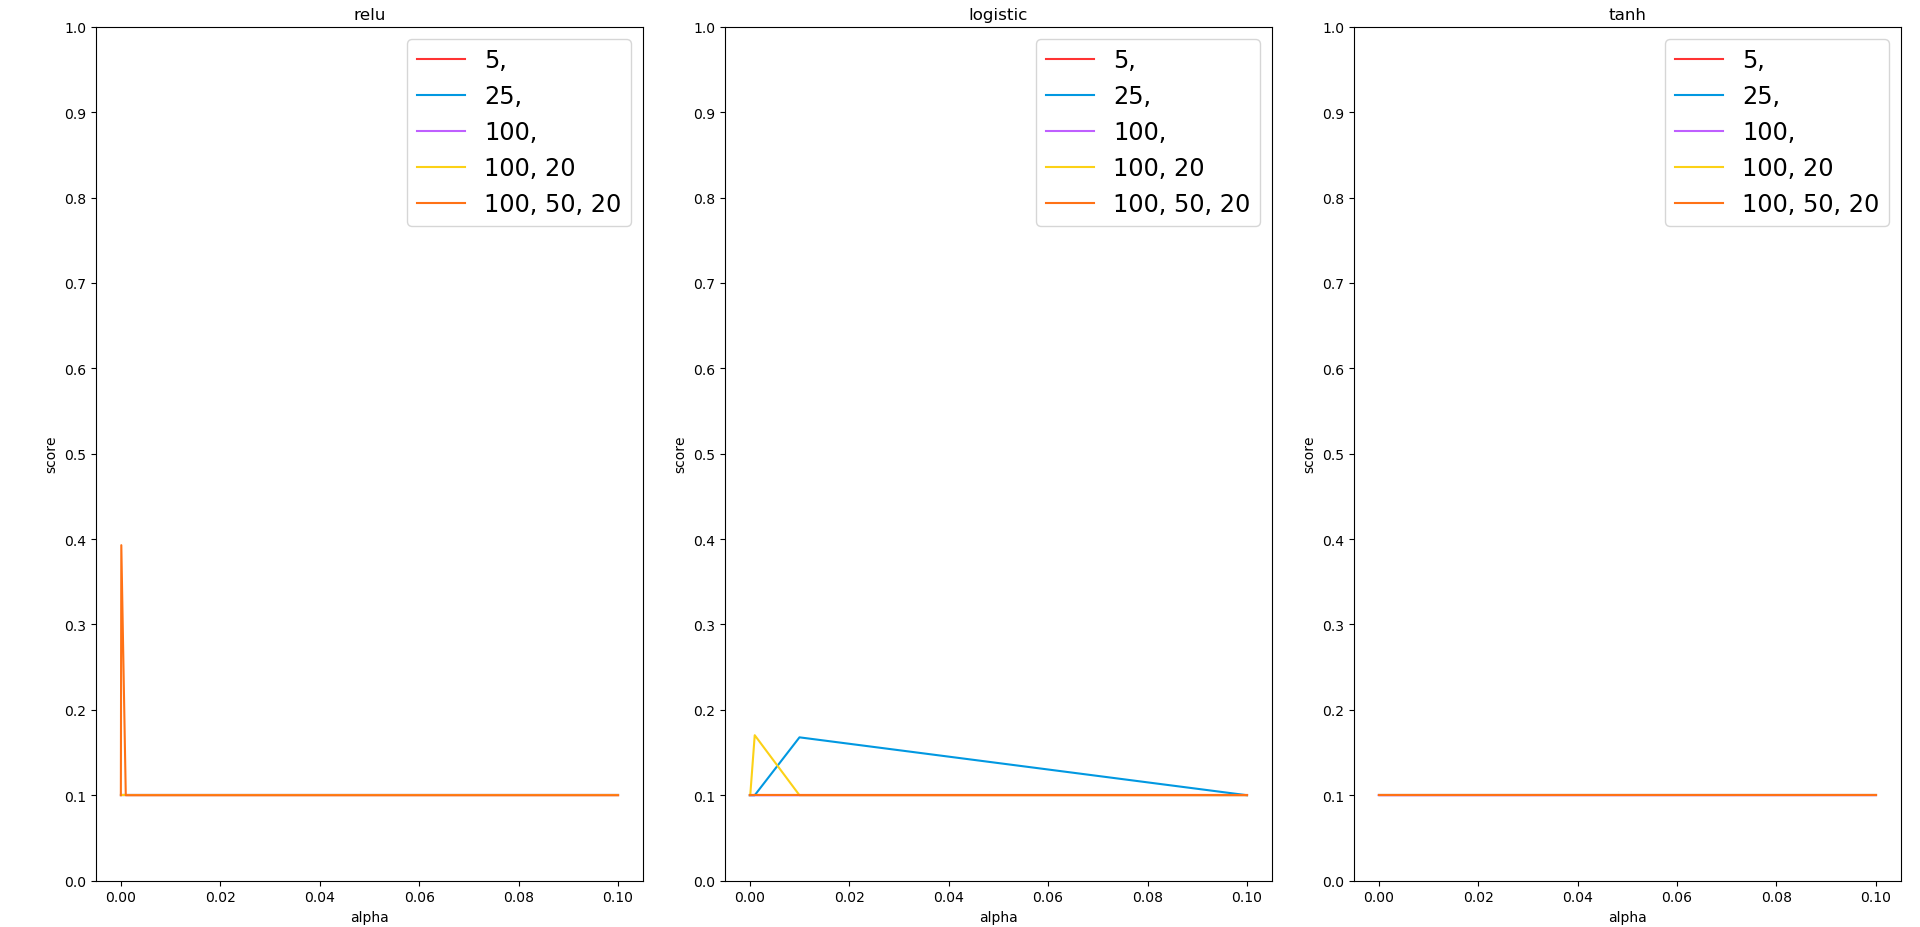
\includegraphics[width=0.5\linewidth]{figure/a2_nn}
				\caption{Colon Cancer数据集上的MLP表现。}
				\label{fig:a2nn}
			\end{figure}
						
			\begin{table}[htbp]
				\centering
				\small
				\caption{Colon-cancer上的准确率比较。}
				\label{tab:mnist}
				\begin{tabular}{lr}
					\toprule
					方法 & 准确率       \\ \midrule
					MLP  & 10\%  \\ %\midrule
					SVM(sigmoid kernel with C=2) 	  & 84\%  \\
					\bottomrule
				\end{tabular}
				\vspace{-5mm}
			\end{table}	
		}
		
		\item[(3)]{
			最后的mnist是著名的手写数字数据集,它是一个被大量测试过的多分类任务数据集。测试了多组SVM参数,最终得到了表\ref{tab:mnist},其中SVM最好的表现是C=0.07时的线性SVM,准确率可以达到94.56\%;进行对比的是一个35个卷积层的神经网络\cite{mnist12}。图\ref{fig:bsvm}展示了各个参数下的SVM的测试结果。
			
			\begin{figure}[htbp]
				\centering
				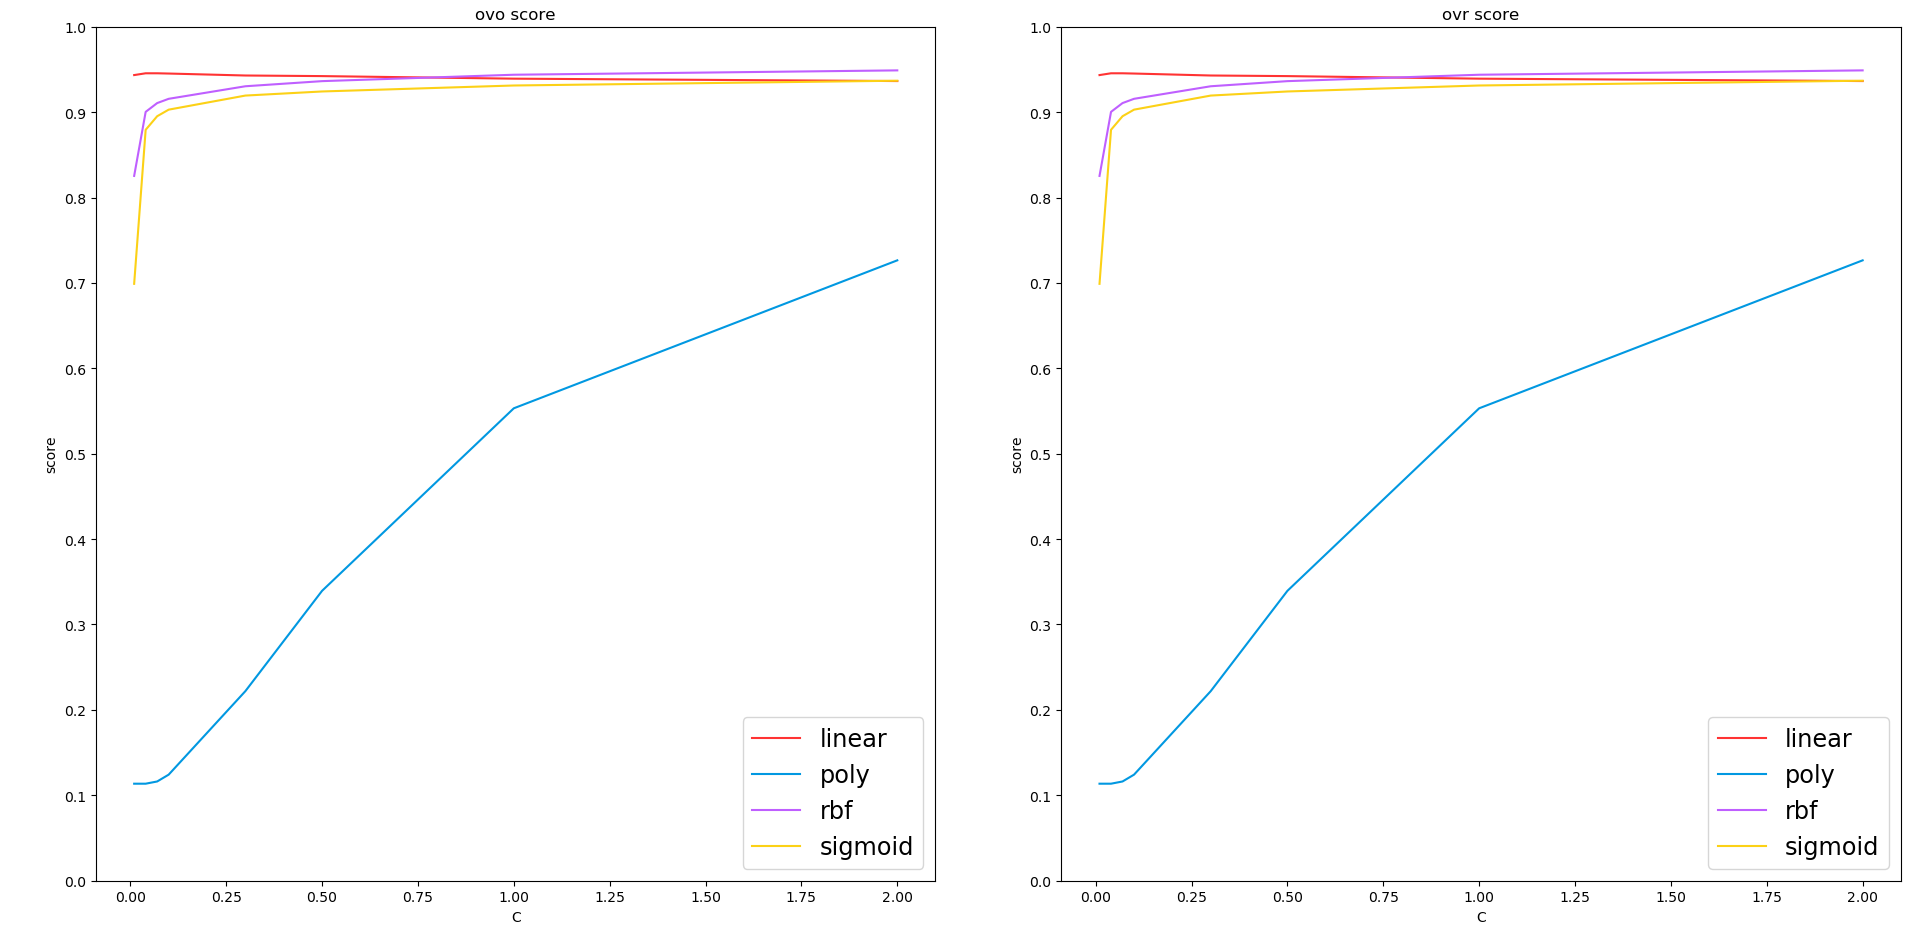
\includegraphics[width=0.5\linewidth]{figure/b_svm}
				\caption{MNIST数据集上的SVM表现。}
				\label{fig:bsvm}
			\end{figure}
		
			\begin{table}[htbp]
				\centering
				\small
				\caption{MNIST上的准确率比较。}
				\label{tab:mnist}
				\begin{tabular}{lr}
					\toprule
					方法 & 准确率       \\ \midrule
					Ciresan et al. CVPR 2012  & 99.77\%  \\ %\midrule
					linear-SVM(C=0.07) 	  & 94.56\%  \\
					\bottomrule
				\end{tabular}
				\vspace{-5mm}
			\end{table}	
			
		}
	\end{enumerate}

	以上数据集实际上都并不大,因此除了这些数据集外,我选取了文档中没有的Animals with Attributes2(AwA2)数据集作为拓展实验\cite{awa2dataset}。该数据集也是zero-shot learning任务中比较经典的一个数据集,提供了50类动物的图片。这里用来做简单的分类学习,虽然该数据集的发布方提供了Resnet50抽取的深度学习特征,为了与Resnet50抽取的特征进行比较,我首先使用Scale-invariant feature transform(SIFT)对图片抽取特征,结果如图\ref{fig:sift}。图\ref{fig:sift}中的绿色点为选取的尺度不变local descriptor,矩形中的绿色向量附近各个区域的梯度方向。之后我使用了Vector of aggregated descriptors(VLAD) 方法对这些local descriptor进行编码。由于一个local descriptor是128维的,VLAD中只保留一阶信息,我设置了$20$个聚类中心,把一张图编码成了$2560$维的向量,作为输入到SVM分类器的特征。SVM使用的是C为0.01的线性SVM,虽然由于这个数据量大只做了一组,但是传统方法是明显落后于深度神经网络的。表\ref{tab:awa2}中展示了分类准确率,我们可以看到,深度神经网络的抽取出的feature做分类,分类的准确率要远高于传统的方法的组合。同时,更为重要的是,深度学习的方法是端到端的过程,无需进行特征的抽取和编码,而使用传统的SVM我们需要人为设计出如SIFT结合VLAD这样的特征抽取系统,显然整体的效果是无法与深度神经网络相比的。

	\begin{figure}[htbp]
		\centering
		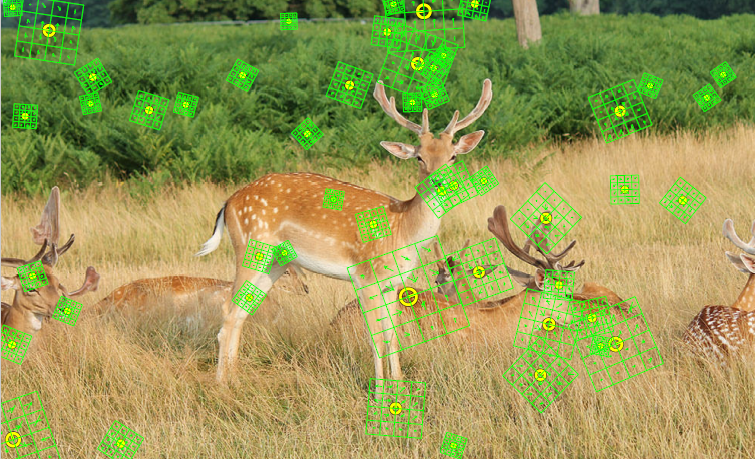
\includegraphics[width=0.5\linewidth]{figure/sift}
		\caption{使用SIFT抽取出的特征。}
		\label{fig:sift}
	\end{figure}

	\begin{table}[htbp]
			\centering
		\small
		\caption{对AwA2数据集的分类准确率。}
		\label{tab:awa2}
		\begin{tabular}{lr}
			\toprule
			方法 & 准确率       \\ \midrule
			Resnet50  & 92.6\%  \\ %\midrule
			SIFT+VLAD+SVM 	  & 26.1\%  \\
			\bottomrule
		\end{tabular}
		\vspace{-5mm}
	\end{table}	

\end{sol}

\end{hw}

\begin{hw}
	Apply one causal discovery algorithm on a real world problem. You need to specify the details of the problem, collect the data by yourself or from a public website, briefly summarize what algorithm you use, and explain the results.
	\begin{sol}
		在现代经济学研究中,一个共识是“国家的股票指数与GDP有着极大的相关性”。如下图\ref{fig:change}所示,二者的变化存在一定时延,但是趋势相同。
		
		\begin{figure}[htbp]
			\centering
			\subfigure[GDP。]{
				\begin{minipage}[t]{0.4\linewidth}
					\centering
					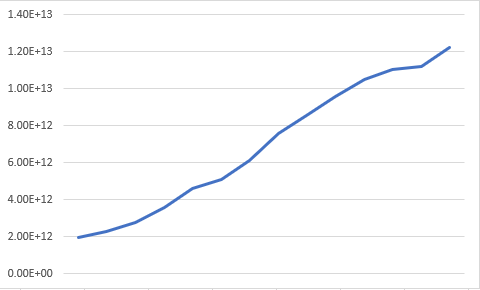
\includegraphics[width=\linewidth]{figure/GDP.png}
					%\caption{GDP.}
				\end{minipage}%
			}%
			\subfigure[沪深300指数。]{
				\begin{minipage}[t]{0.4\linewidth}
					\centering
					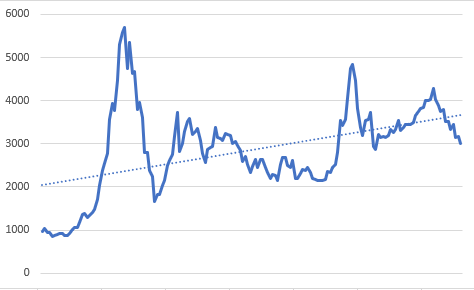
\includegraphics[width=\linewidth]{figure/stock.png}
					%\caption{沪深300指数。}
				\end{minipage}%
			}%
			\centering
			\caption{中国GDP和沪深300指数变化曲线。}
			\label{fig:change}
		\end{figure}
	
		股指在一定程度上折射出了企业盈利状况和投资人对市场的信心,因而股指可以与GDP共同反映出一个国家经济的基本情况。美国股市自08年经济危机以来,总体上保持了近十年的牛市,带给了特朗普对国内经济的信心,这也是他敢于打响中美贸易战的一个重要因素。
		
		然而,虽然二者间的相关性是公认的,但是二者的因果关系却不是很明朗。虽然从图\ref{fig:change}中也可以看到,二者的变化有明显的先后关系,但是经济学家仍然无法确定是GDP上升导致了股指上升,还是股指上升导致了GDP增长。我在本次作业中选取了全球主要国家从2005年到2017年共13年间的GDP和股指的数据。
		
		下表\ref{tab:country}为选取的国家及股指名称,数据来源于\cite{financial,worldbank}:
		\begin{table}[htbp]
			\centering
			\small
			\caption{国家及对应选取的股指。}
			\label{tab:country}
			\begin{tabular}{lr}
				\toprule
				国家 & 股指     \\ \midrule
				中国(China)  & 沪深300 \\ %\midrule
				美国(United State) & 标普500  \\ %\midrule
				澳大利亚(Australia)    &  澳大利亚标普200 \\ %\midrule 
				德国(Germany)  & 德国DAX \\
				巴西(Brazil)  & 巴西BOVESPA \\ %\midrule
				印度(India)  & 印度孟买30 \\ %\midrule
				英国(United Kingdom) & 英国富时100 \\ %\midrule
				加拿大(Canada)  & 加拿大标普\\
				\bottomrule
			\end{tabular}
			\vspace{-5mm}
		\end{table}	
	
	由于数据的规模并不大(共八个国家,每个国家13年),我尝试了多种分析方法以提高准确性,同时可以比较各个方法。
	
	首先是经典的线性非高斯因果模型(Lingam),在因果推断中,一个难点在于如何在模型中建立有向性,一般的线性模型自变量与因变量可以交换地位,二者均可以互相表示,无法区分因果,Lingam借鉴了独立成分分析(ICA)的思路,使用了非高斯分布的变量进行线性组合,从而与ICA类似确定唯一的表示\cite{causal}。在给定数据集上,分析结果如图\ref{fig:lingam},可以看到,对任意一个国家,均为股票市场变动是因,GDP是果。
	
	之后我又尝试了igci模型,igci模型添加一个假设来使得因果关系是单向的,它假设输入的分布和因果机制之间是独立的,利用information space的正交性来区分因果\cite{igci}。结果如图\ref{fig:lingam},此时分析结果与Lingam模型出现了不一致之处,对于一些国家,GDP变动是因,而一些国家GDP变动为果。这可能与国家的经济政策有关,也可能是样本集合太小,但是历史的股票指数数据很难收集,不便于扩充数据集。
	
	最后我尝试了文档中推荐的Tetrad软件,该软件集成了大量因果推断算法,且拥有友好的图形界面。在图\ref{fig:prj}中,我首先绘制了一幅图来表示Structure equation model(SEM),同时使用了两种算法FCI和FASK。FCI算法歧视很类似著名的PC算法,增加了一些限制条件对可以表示因果关系的有向无环图进行搜索。它有两个阶段,第一个阶段先建立一个完整的无向图,执行一系列条件独立性测试,以消除无向图中两个相邻变量之间的边。在删除一些无关的边后,在该无向图的基础上,使用算法添加的条件,进行定向操作,尽可能多得定向。FASK也是一个PC算法的变种,它搜索图中要用于定向的邻接节点\cite{tetrad}。
	推断结果在图\ref{fig:fci}和\ref{fig:fask}中。可以看到FCI中的结果认为二者有公共的未观测到的干扰因子使得无法得到明确的结论,而FASK中则认为股票是因,GDP是果。
	
	\begin{figure}[htbp]
		\centering
		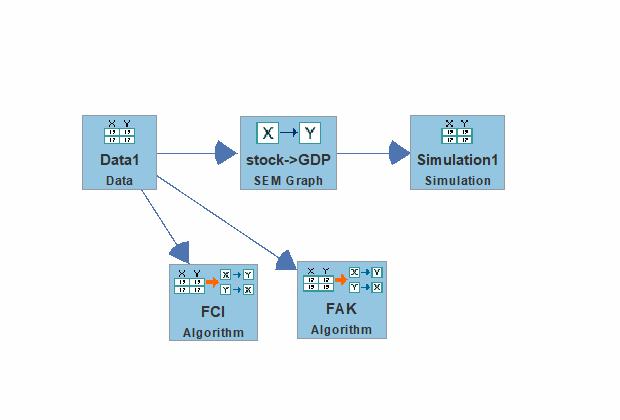
\includegraphics[width=0.5\linewidth]{figure/prj}
		\caption{Tetrad绘图。}
		\label{fig:prj}
	\end{figure}

	
	\begin{figure}[htbp]
		\centering
		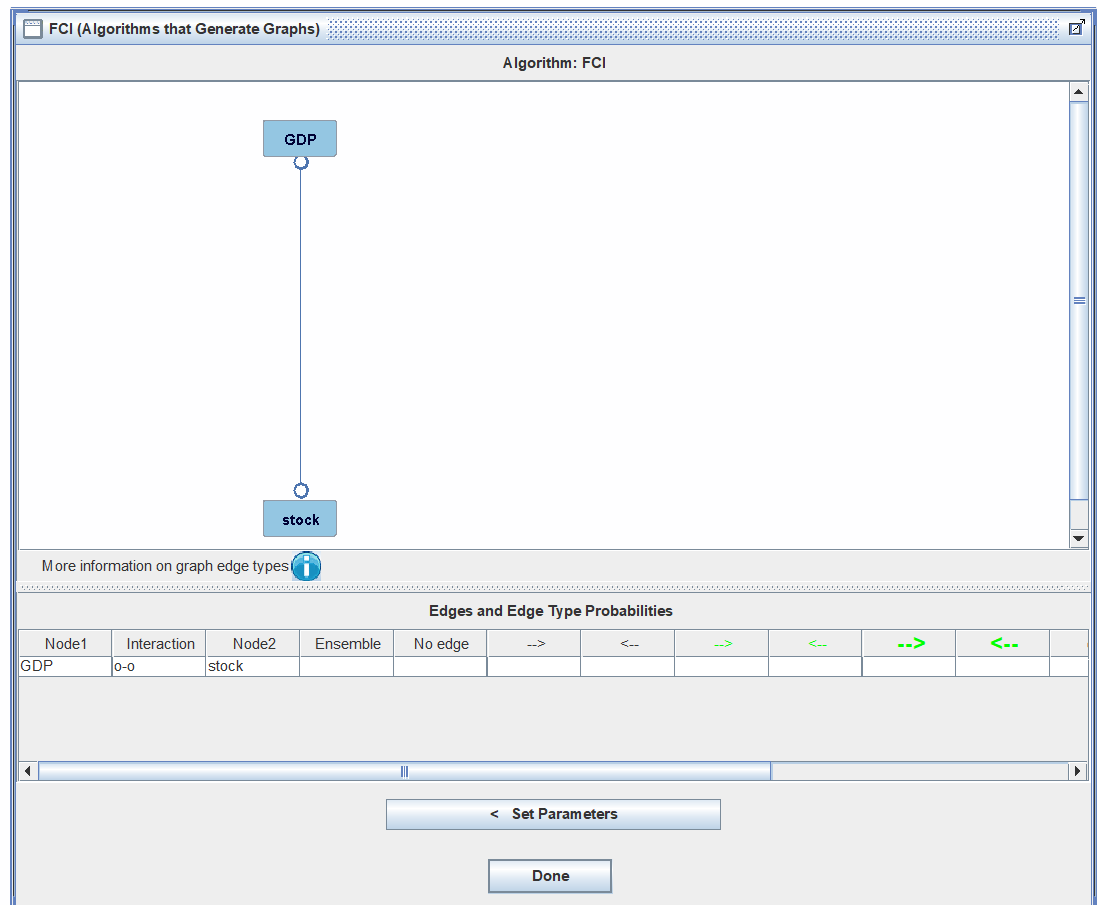
\includegraphics[width=0.5\linewidth]{figure/FCI}
		\caption{FCI结果。}
		\label{fig:fci}
	\end{figure}
	
	\begin{figure}[htbp]
		\centering
		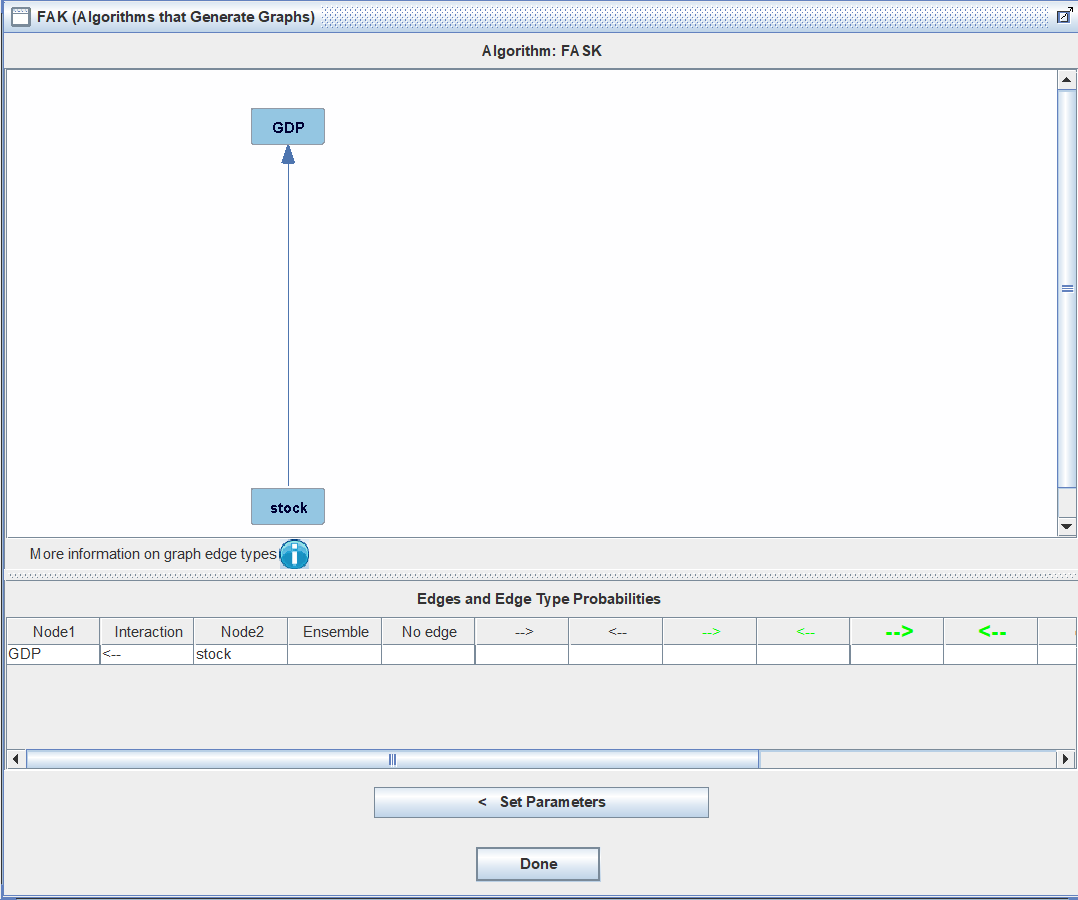
\includegraphics[width=0.5\linewidth]{figure/FASK}
		\caption{FASK结果。}
		\label{fig:fask}
	\end{figure}

	综合多种算法的结果,我们可以初步得出结论,GDP与股票指数是具有很强的相关性的,甚至因果关系也很明显,可以认为股指的涨跌可以导致GDP的涨跌,即可以根据股票市场对GDP作出预测。事实上,从经济学的角度来分析,这也是合理的,当股票指数增长时,可以看出企业盈利能力明显增强,投资人信心日益增长,同时政府也可能采取了宽松的货币政策导致市场上的流动的货币数量增加,这一切都可以视作GDP增长的信号。反之,当市场低迷时,国民生产总值的增长也就如空中楼阁,无从谈起。
	\end{sol}
\end{hw}

\bibliographystyle{plain}
\bibliography{report}

\end{document}